% SPDX-License-Identifier: Apache-2.0
\documentclass[11pt,a4paper]{article}
\usepackage[margin=23mm,headheight=15pt]{geometry}
\usepackage[T1]{fontenc}
\usepackage[utf8]{inputenc}
\usepackage{lmodern,microtype,amsmath,amssymb,graphicx,booktabs,longtable,tabularx,array}
\usepackage{xcolor,tikz,tcolorbox,enumitem,fancyhdr,titlesec,caption,float}
\usepackage[numbers,sort&compress]{natbib}
\usepackage{xurl}
\usepackage{hyperref}
\definecolor{ink}{HTML}{201631}
\definecolor{purple}{HTML}{6135B4}
\definecolor{deep}{HTML}{180D32}
\definecolor{lavender}{HTML}{ECE5F8}
\definecolor{mint}{HTML}{1B7764}
\definecolor{muted}{HTML}{625B70}
\definecolor{gold}{HTML}{C49D59}
\hypersetup{colorlinks=true,linkcolor=purple,citecolor=purple,urlcolor=purple,pdftitle={AGI ALPHA FLYWHEEL: The Productive Capital Engine},pdfauthor={MONTREAL.AI research edition},pdfsubject={Useful digital work, conserved cash, capability investment and measured reuse}}
\urlstyle{same}
\setlength{\parindent}{0pt}
\setlength{\parskip}{5.5pt}
\setlength{\emergencystretch}{2em}
\renewcommand{\arraystretch}{1.18}
\setlist{nosep,leftmargin=1.4em,topsep=4pt}
\captionsetup{font=small,labelfont=bf}
\titleformat{\section}{\Large\bfseries\color{purple}}{\thesection}{0.7em}{}
\titleformat{\subsection}{\large\bfseries\color{ink}}{\thesubsection}{0.6em}{}
\pagestyle{fancy}
\fancyhf{}
\fancyhead[L]{\small\color{muted}AGI ALPHA FLYWHEEL}
\fancyhead[R]{\small\color{muted}THE PRODUCTIVE CAPITAL ENGINE}
\fancyfoot[L]{\small\color{muted}Independent research edition \textbullet\ 25 October 2026}
\fancyfoot[R]{\small\thepage}
\renewcommand{\headrulewidth}{0.3pt}
\newtcolorbox{finding}[1]{colback=lavender,colframe=purple,boxrule=0.5pt,arc=2mm,title={#1},fonttitle=\bfseries,coltitle=white,left=3mm,right=3mm,top=2mm,bottom=2mm}
\newcommand{\obs}{\textsf{Observed}}
\newcommand{\modl}{\textsf{Modeled}}
\newcommand{\nr}{\textsf{NOT RUN}}
\newcommand{\code}[1]{\texttt{\small #1}}
\newcommand{\StudyRuns}{72}\newcommand{\FamilyChecks}{216}

\begin{document}
\hypersetup{pageanchor=false}
\begin{titlepage}
\begin{tikzpicture}[remember picture,overlay]
\fill[deep] (current page.south west) rectangle (current page.north east);
\fill[purple,opacity=.25] ([xshift=3cm,yshift=-5cm]current page.north east) circle (7cm);
\draw[gold,opacity=.65,line width=.5pt] ([xshift=2.3cm,yshift=-3.2cm]current page.north west) -- ([xshift=-2.3cm,yshift=-3.2cm]current page.north east);
\foreach \x/\y in {2/3,4/1,8/4,11/2,14/6,17/3,18/10,5/16,15/19,3/22,18/25,12/24}{\fill[white,opacity=.35] ([xshift=\x cm,yshift=-\y cm]current page.north west) circle (.6pt);}
\end{tikzpicture}
\color{white}
\vspace*{1.2cm}
{\large\sffamily MONTREAL.AI \hfill RESEARCH / 2026}\par
\vspace{2cm}
{\Large\sffamily AGI ALPHA FLYWHEEL}\par
\vspace{0.6cm}
{\fontsize{39}{48}\selectfont\bfseries The Productive\\Capital Engine\par}
\vspace{0.8cm}
{\Large From Valuable Work to\\Expanding Productive Capability\par}
\vspace{1.3cm}
{\large Useful work. Conserved cash. Earned capability.}\par
\vfill
\begin{minipage}{.85\linewidth}
\large Can useful digital work generate a defensible operating surplus, and can that surplus finance capabilities that improve subsequent production?
\end{minipage}
\vspace{1.4cm}\par
{\large\bfseries SUCCESSOR $\Omega$ HARNESS}\par
{\sffamily ACTIVATE. EVOLVE. SCALE.}\par
\vspace{0.3cm}
{\small Powered by TRANSFORMATIONAL INTELLIGENCE $\infty$\\and the applicable \$AGIALPHA utility.}\par
\vspace{1.0cm}
{\small Independent additive study \textbullet\ 25 October 2026\\Native research execution and explicit economic scenarios.}
\end{titlepage}
\setcounter{page}{1}
\hypersetup{pageanchor=true}
\section*{Abstract}
The immediate commercial question for AGI ALPHA is whether an accepted digital deliverable offers useful value at an attractive complete cost relative to competent traditional human work. A second question concerns the enterprise: how much of that value can it retain as spendable surplus, and what productive capability can that surplus finance? These questions require different evidence. Low kernel runtime establishes neither a cheap complete service nor a self-financing enterprise.

We implement an additive production-and-reinvestment study around the existing SUCCESSOR workbench and planning components. Three connected services produce source/dependency inventory assurance, a resource-constrained rollout plan and a bilingual evidence-linked dossier. A retained predecessor index and a distinct dependency-aware repair capability connect initial work to changed work. A prospectively frozen local evaluation preserves conventional full rebuild and equivalent caching comparators, rejected constructions and unsupported inputs. Official labor sources supply wage and employer-cost anchors; unobserved human task duration is represented by break-even thresholds. A conserved financial model separately traces prices, actual-or-modeled collections, delivery costs, reserves, working capital and discrete capability investment under 0\%, 25\%, 50\% and 75\% allocation policies.

The original campaign accepted 72/72 joint outputs across six controlled projects, with 24 parent invocations and 12 child invocations. It demonstrates source-bound reuse, but the flywheel consumed 0.9\% more CPU than ordinary caching on fresh changes and expanded no verified same-budget frontier. A separately frozen correction passed 28 finite edge cases after adversarial review found real input-boundary defects. Under explicit U.S. compensation, price and attention assumptions, modeled complete costs are USD28.26--35.16 per accepted service. Customer purchase break-even times are approximately 60, 79 and 57 traditional minutes for the three classes; actual matched durations remain unknown. The six-cycle direct-sale scenario retains USD8,776 of earned cash after its obligation reserve. That amount covers 2.46 times the specified next plan's cash need, but the plan fails the unchanged operating-spend ceiling. A separately labeled smaller-plan diagnostic is feasible. The measured repair capability remains an investment HOLD because the conventional incumbent is cheaper. Self-financing and self-acceleration are not demonstrated.


No customer payment, authenticated browser-to-approved-executor run or matched human trial was observed. Monetary results are scenarios informed by execution and source evidence. The study distinguishes an implementable financing mechanism, financially fundable construction, economically justified investment and self-acceleration. These are separate claims.

\begin{finding}{Commercial foundation}
Offer valuable work where its full cost and quality justify the customer's purchase. Use subsequent evidence to decide which capabilities deserve the surplus. A useful business does not require a prior demonstration of self-acceleration.
\end{finding}

\section{Contribution and claim boundaries}
\label{sec:contribution}
An accepted job can produce three different assets: a customer deliverable, a reusable operational artifact and cash. None is automatically the other. The customer's avoided labor expense is not enterprise revenue; a reusable script is not an improvement until its reuse is useful; and an invoice is not collected cash. This study joins these assets through inspectable records without collapsing their meanings.

The contribution is an executable, conserved connection between production and a specified next investment. It is distinct from the Economics writer's 42-job portfolio and separately frozen operational-economics amendment. It does not replace those studies, the Software Capability Foundry, Strategy Succession or their negative findings. The inspected Alpha main is \code{f836f06e}; exact full commit identities for all four repositories are preserved in the source ledger. Additive coordination is recorded in issue 4850.\citep{alpha_source,coordination}

The main questions are: (Q1) Can the declared workflows produce accepted, useful deliverables? (Q2) Under what complete-cost and human-time conditions are they commercially attractive? (Q3) What cash remains after obligations and reserves? (Q4) Can it finance a specified capability and its next use? (Q5) Does the capability improve costs, quality or supported work after construction and maintenance? Q1 is evaluated locally; Q2--Q4 are explicitly conditional where their inputs are not observed. Q5 combines measured technical effects with separately labeled cost assumptions.

\begin{table}[H]\small\centering
\begin{tabularx}{\linewidth}{p{.23\linewidth}X}
\toprule Claim & Evidence required \\\midrule
Useful delivery & Inspectable artifact and declared acceptance checks. \\
Commercial advantage & Matched deliverable quality, complete Agent cost and a credible traditional alternative. \\
Self-financing & External collections sufficient after obligations, losses and reserves. \\
Capability improvement & Changed subsequent production under a consistent evaluation slice, net of costs. \\
Self-acceleration & Improvement in the process that creates improvements, measured over successive generations after its own costs. \\\bottomrule
\end{tabularx}
\caption{A higher claim requires additional evidence. Rising cumulative output is sufficient for none of the last three rows.}
\end{table}

\section{Sources, architecture and historical evidence}
\label{sec:architecture}
\subsection{One mission history; separate authority}
The seven stages of TRANSFORMATIONAL INTELLIGENCE become concrete provenance records. Computation precedes their checkpoint serialization; these records do not establish separately enforced or independently timed seven-stage execution. Identify produces scope and acceptance; Out-Learn supplies source provenance; Out-Think analyzes dependencies and alternatives; Out-Design constructs an artifact or repair; Out-Strategise selects a bounded method and resource allocation; Out-Execute records delivered files and checks; Out-Evolve records retention and subsequent invocation. The study reuses the existing workbench instead of creating a competing scheduler.\citep{transformational,alpha_source}

Alpha supplies workbench history, content identities and bounded planning. Manager supplies the separate USDC route and job-specification semantics. Jobs v0 supplies the distinct AGIALPHA settlement and incentive route. Fleet supplies source-bound handoff and execution/review boundaries. Local workbench serialization or a valid artifact is not remote Fleet execution. The inherited generic job charter is an aggregation-oriented scaffold; the separate source/schedule/dossier oracle supplies this study's acceptance. Those interfaces are mapped where applicable; a transaction is not introduced merely to claim use of a repository. The local companion neither provisions a signed journal nor changes approved executors, deployed contracts, credentials or security settings.\citep{manager_source,jobs_source,fleet_source}

\begin{figure}[H]\centering
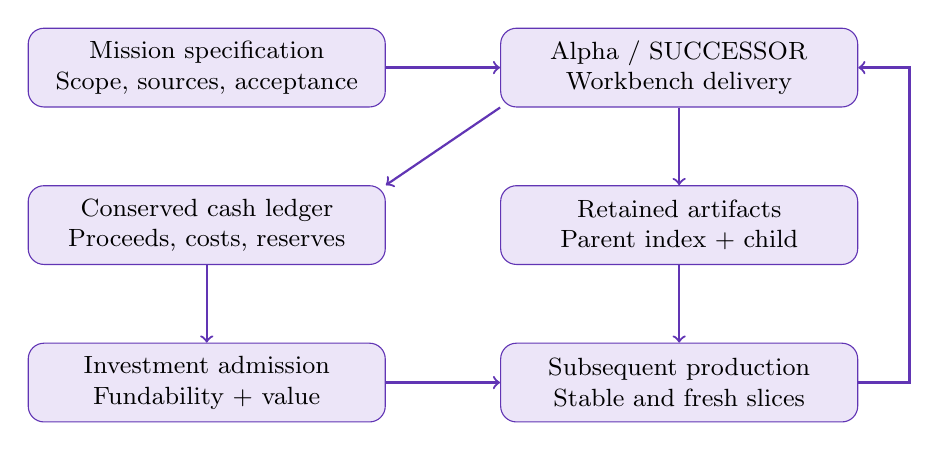
\begin{tikzpicture}[every node/.style={font=\small,align=center},box/.style={draw=purple,fill=lavender,rounded corners=2mm,text width=4.3cm,minimum height=1.0cm},arr/.style={->,thick,color=purple}]
\node[box] (mission) at (0,0) {Mission specification\\Scope, sources, acceptance};
\node[box] (delivery) at (6,0) {Alpha / SUCCESSOR\\Workbench delivery};
\node[box] (retained) at (6,-2) {Retained artifacts\\Parent index + child};
\node[box] (ledger) at (0,-2) {Conserved cash ledger\\Proceeds, costs, reserves};
\node[box] (invest) at (0,-4) {Investment admission\\Fundability + value};
\node[box] (next) at (6,-4) {Subsequent production\\Stable and fresh slices};
\draw[arr] (mission)--(delivery);\draw[arr] (delivery)--(retained);\draw[arr] (delivery.south west)--(ledger.north east);
\draw[arr] (ledger)--(invest);\draw[arr] (retained)--(next);\draw[arr] (invest)--(next);
\draw[arr] (next.east)--++(.65,0)|-(delivery.east);
\end{tikzpicture}
\caption{Implemented local artifact links and a separately modeled financial link. Manager, Jobs and Fleet retain their distinct settlement/admission boundaries; no transaction or external execution is implied by the diagram.}
\end{figure}


\subsection{Strategy Laboratory and prior negative findings}
The supplied Strategy Laboratory motivates better method construction: decomposition, evidence acquisition, routing, minimal repair, reusable intermediate assets and allocation of review. Its archived description is a bounded evolutionary prototype with fixed evaluators and fresh-task confirmation. The present commission recovered the public provenance and audit projection, but the original DOCX bytes were not available through the supplied file context. We therefore distinguish freshly verified repository artifacts from historical reports about the original DOCX and 62-payload archive. We do not claim to have re-read unavailable original bytes.\citep{strategy_history}

Historical Strategy Succession remains unchanged: 517/864 qualified outcomes for the primary flywheel, tied with the equally funded learner and below the stronger fixed portfolio's 591; no primary retained asset; no fresh repair that both invoked its parent and qualified. The later engineering repair retained a native movement cost of 7 against the constructed candidate's 9. Source-linked verification details, the precise replication scope and original identities appear in the companion.\citep{strategy_results,strategy_worker}

These observations motivate a strong incumbent and an explicit admission decision. A criticism must identify a reproducible violated constraint or a sourced mismatch before it changes an output. An unevidenced adversarial assertion does not override a checked result. A conventional solution may remain the best production choice even when lineage and reuse are technically functional.

\section{Prospective design and implemented services}
\label{sec:design}
\subsection{Selection, complexity and coverage}
We select complementary services that can form a complete release-change workflow. A release assurance packet identifies components, hashes, dependencies and evidence. A rollout plan assigns finite jobs under precedence, duration and resource limits. A bilingual dossier explains the checked release and its change history to an operator or stakeholder. These outputs have different acceptance conditions and are reported by class. They are not interchangeable units of value.

Selection requires public or synthetic nonpersonal inputs, inspectable acceptance, a plausible traditional occupation, meaningful dependencies or revisions and a feasible local execution path. The evaluation contains multiple contexts and complexity strata. Generated projects are controlled research instances; they are not a representative random sample of commercial customers. No result is extrapolated to arbitrary software repair, open-ended research or universal digital work.

\begin{table}[H]\small
\begin{tabularx}{\linewidth}{p{.24\linewidth}X}\toprule Design element & Prespecified content \\\midrule
Projects & SDK release, research publication and operations handoff; each with simple and complex strata. \\
Inputs & 14 exact public source snapshots. Declared dependencies, durations, resource calendars and revisions are synthetic. \\
Complexity & Simple: 8 components and 6 jobs. Complex: 14 components and 12 jobs. \\
Cycles & Initial production; stable replay; fresh source/duration revision; fresh edge/calendar change and repair. \\
Alternatives & Full rebuild, predecessor/child flywheel and independently written conventional dependency-key caching. Existing Alpha portfolio and native specialists remain available. \\
Counts & Six project instances $\times$ four cycles $\times$ three arms = 72 joint executions, each with three deliverable checks (216 checks). These are not 216 independent jobs. \\
Bounds & 18 components, 18 planning jobs, 128 slots, 4 crew; 2-second native solves, 30-second Node process timeout. \\
Freeze & 38 files; 25 October 2026, 14:14:23 UTC. Full identities and subsequent correction boundary are in the companion. \\\bottomrule\end{tabularx}
\caption{One controlled connected-production experiment, with stable and fresh slices.}
\end{table}


\subsection{Retention, fresh change and child construction}
The parent retains a content-addressed dependency and evidence index after accepted work. A fresh source or dependency change tests whether old artifacts remain valid. The child computes transitive invalidation and constructs a coherent change/repair packet, invoking the parent and preserving unchanged evidence. Direct-only invalidation is a deliberately explored developmental strategy whose failure remains charged and visible when a transitive dependency changes.

Full rebuild remains available. An ordinary equivalent caching method remains available. This is essential: savings against wasteful reconstruction do not establish an advantage over conventional reuse. The child is an authored software capability, not evidence of autonomous algorithm invention. Any newly supported cross-artifact certificate is an expansion of the declared interface. Practical expansion under the same budgets requires separate acceptance and budget evidence; the absence of a button in an incumbent is not proof of computational impossibility.

\subsection{Freeze, held-out slices and acceptance}
Development cases precede the freeze. The frozen boundary binds task generation, implementation, acceptance and analysis before held-out inputs are generated. A consistent slice tests repeat production and a separate fresh-change slice tests transfer and changed requirements. Exact raw records include arm, task, cycle, input/output hashes, parent invocations, work accounting, resource measurements, errors and acceptance. Source custody is shared within this research session; the held-out split prevents result-driven retuning but does not provide blind external custody.

Acceptance checks source completeness, transitive consistency, valid provenance, schedule feasibility and dossier agreement with the checked facts. A separate checker is used where the existing runtime supplies it. Rejection, timeout and unsupported input are preserved. Machine acceptance does not establish a paying customer's editorial satisfaction or legal suitability. These remaining checks enter the economic envelope as explicit human work.

\section{Measured production and capability effects}
\label{sec:production}
The original frozen campaign recorded 72/72 joint results accepted by its declared oracle, corresponding to 216/216 family acceptance checks. Within each treatment, each class has 24 accepted outputs across six projects and four cycles. No retries were needed on these supported inputs; four separately counted refusal controls rejected cyclic dependencies, missing evidence, private data and job-count overflow. There were 24 observed parent invocations and 12 child invocations. These counters establish use, not economic benefit.

The stable repeat reduced six-project CPU from \textbf{2.271 seconds} for full rebuild to \textbf{0.845 seconds} for the flywheel, while conventional caching used \textbf{0.822 seconds}. On the two fresh-change cycles, flywheel and conventional caching each rebuilt only \textbf{18 of 132 source cards} and reused 114. Their total CPU was \textbf{4.069} and \textbf{4.033 seconds}, respectively. The flywheel was approximately \textbf{0.9\% slower} on this recorded fresh slice. Six local instances do not establish a population timing difference; they establish no demonstrated superiority over the strong incumbent.

\begin{figure}[H]\centering\includegraphics[width=\linewidth]{figures/production.pdf}
\caption{Recorded native research. CPU includes the joint local pipeline, native/portfolio planning, checks and persisted artifacts; it is not complete Agent cost. The source-card reduction is also achieved by ordinary caching. Each point summarizes six controlled projects.}\end{figure}

\begin{table}[H]\small\centering\begin{tabular}{lrrr}\toprule Cycle & Full rebuild CPU (s) & Flywheel CPU (s) & Cache CPU (s)\\\midrule
Initial & 2.337 & 2.451 & 2.489 \\
Stable repeat & 2.271 & 0.845 & 0.822 \\
Source/duration change & 2.401 & 2.369 & 2.273 \\
Dependency/calendar repair & 1.674 & 1.700 & 1.760 \\
\bottomrule\end{tabular}\caption{Observed joint CPU; one cost belongs to three deliverables and is not counted three times.}\end{table}

Observed median local wall times for a joint flywheel request were 361.9, 122.0, 360.1, 230.0 milliseconds for the initial, stable, source-change and dependency-change cycles, respectively. They exclude unmetered authoring, human review, customer communication and the unavailable live executor path. No active human-minute measurement is available.

Child descriptor construction across six bindings consumed 0.421 seconds wall time and 0.466 seconds CPU in addition to service execution. These measurements cover authored-algorithm binding and checking, not the human/model effort that designed or corrected the algorithm. Original initialization, developmental failures and refused inputs are retained separately.

\subsection{Post-freeze defects and the corrective edition}
Independent-role adversarial review after the original freeze found stale path-only metadata, cross-project predecessor reuse, inadequately checked construction origin and inconsistent deletion handling. The original oracle also failed some tampered metadata/digest probes. Those controls were outside the original fixed-inventory confirmation inputs. The original acceptance totals are preserved with that scope; they do not qualify arbitrary changed projects. A separately frozen corrective adapter and fresh edge evaluation are reported below. No historical result was overwritten or promoted to the new source identity.

The corrective v1.1 adapter uses path- and provenance-aware content keys, rejects cross-project predecessors, checks immutable construction origin and preserves an accepted child registry for subsequent use. After developmental review, its own freeze bound 36 files at 14:19:54 UTC. A fresh qualification then produced \textbf{25 accepted outputs and three expected refusals}: \textbf{28/28 cases passed}, with 3,265 strengthened Python assertions. A separately authored saved-output audit passed 3,885 assertions. These finite edge cases qualify the correction only within their scope; they do not replace the original 72-run timing campaign or establish general correctness. The browser demo uses v1.1. The economic measurement bridge retains the original scoped timing results without claiming corrected timing superiority.


The new change-impact and cross-artifact certificate is a real implemented interface. The strong conventional alternatives can produce the same deliverables under the declared bounds. Consequently, \textbf{previously impractical work becoming feasible under the same budgets is not established}. Discovery-process improvement and self-acceleration are also not established.


Resource measurements include local wall time, CPU when available, operation counts and artifact bytes. They are scoped to the recorded environment. Microtimings are not stable cross-device performance guarantees. A named work unit measures an implementation action; it is not a dollar, a human minute or a physical instruction. Setup, authorship, prompt/model use, verification, failed constructions and maintenance cannot be priced from these counts alone.

The full authenticated service path remains \nr. The research does not convert an offline browser action into a live executor receipt. It also does not claim continuous operation after browser closure, independent human review or external demand. The demo visibly separates fresh local computation, recorded confirmation and financial simulation.

\section{The immediate human-work comparison}
\label{sec:human}
\subsection{Competent ordinary-tool work}
The primary commercial alternative is a competent worker using ordinary non-AI software. That includes existing scripts, test runners, spreadsheets, document templates and conventional optimizers. It does not require manual enumeration of a task that an existing tool already solves. Wage surveys establish an hourly cost anchor, not a task duration or identical quality. Their populations do not reliably disclose AI use; the modeled comparator therefore combines sourced compensation with an explicitly ordinary-tool task assumption.

The current BLS occupation pages report May 2025 annual medians of USD135,980 for software developers, USD88,940 for operations-research analysts and USD90,390 for technical writers. A reconciliation-clerk anchor is retained for the wider market map. June 2026 private-industry ECEC reports wage costs of USD32.82 plus benefits of USD14.07, totaling USD46.89 per hour. Applying the aggregate benefit factor to occupation medians is a modeled loading, not observed occupation-specific compensation.\citep{bls_software_2025,bls_operations_2025,bls_writer_2025,bls_bookkeeping_2025,bls_ecec_2026q2,bls_oews_method}

\begin{table}[H]\small\centering\begin{tabular}{lrrr}\toprule Occupation / use & Annual wage (USD) & Wage/hour & Loaded scenario/hour\\\midrule
Software / assurance & 135,980 & 65.38 & 93.40 \\
Operations / planning & 88,940 & 42.76 & 61.09 \\
Technical writing / dossier & 90,390 & 43.46 & 62.09 \\
Clerical reconciliation (scope) & 50,670 & 24.36 & 34.80 \\
\bottomrule\end{tabular}\caption{Sourced May 2025 U.S. medians; calculated hourly anchors use 2,080 hours and the estimated benefit factor $46.89/32.82$. No task duration is inferred.}\end{table}

\begin{table}[H]\small\centering\begin{tabular}{lrrrr}\toprule
Service & Full cost & Price & Production BE & Purchase BE \\\midrule
Source assurance & 28.26 & 90.00 & 18.2 min & 59.8 min \\
Rollout planning & 35.16 & 75.00 & 34.5 min & 78.7 min \\
Bilingual dossier & 32.93 & 55.00 & 31.8 min & 57.1 min \\
\bottomrule\end{tabular}\caption{USD and minutes. All Agent costs and prices are modeled, not invoices or observed live costs. Production break-even uses cost; purchase break-even includes price plus assumed customer review. Competent ordinary-tool human duration and matched customer quality remain unmeasured.}\end{table}
At an assumed 30-minute traditional duration, none of the three customer offers is cheaper. At 60 minutes, source assurance and the dossier are slightly cheaper, while planning remains more expensive. At 120 minutes, all three offers provide modeled customer savings. These are decision thresholds, not measured task-time claims. A small simple case may be faster for a competent worker than its headline occupational wage suggests.

The experiment executes three outputs jointly. The financial model assumes a market in which these classes can be ordered and priced separately, assigning one third of joint native CPU to each class and adding class-specific human attention. This is a commercial packaging assumption, not observed separability or a measured market mix. Native CPU is tiny in the total; attention and setup dominate. The model therefore cannot support a USD0.50 complete-service claim.

\begin{figure}[H]\centering\includegraphics[width=\linewidth]{figures/commercial.pdf}
\caption{Conditional customer comparison, using sourced compensation and explicitly assumed ordinary-tool duration. The horizontal lines include price and customer review. Intersections are purchase break-even times; no human completion time was observed.}\end{figure}


O*NET occupational profiles support the relevance of testing, planning, reconciliation and technical communication. ILOSTAT definitions distinguish earnings from total employer labor cost. Eurostat and Canada's Job Bank provide separate geography/currency anchors; neither is converted silently into U.S. dollars. These sources support sensitivity and scope, not a claim of worldwide price equivalence.\citep{onet_software_2026,onet_operations_2026,onet_writer_2026,onet_bookkeeping_2026,ilostat_wages_method,eurostat_labour_2025,jobbank_writer_2024}

\subsection{Two break-even times}
Let $W_H$ be the traditional worker's modeled loaded hourly rate and $C_A$ the complete cost per accepted Agent deliverable, including failed attempts and allocated setup. The production-cost break-even time is
\begin{equation} t^*_{\mathrm{production}}=60C_A/W_H. \end{equation}
The customer's purchase threshold is different. For price $P$, customer review time $h_C$ in hours, customer attention rate $W_C$ and switching expense $S_C$,
\begin{equation} t^*_{\mathrm{purchase}}=60(P+W_Ch_C+S_C)/W_H. \end{equation}
Numerical scenarios set switching expense $S_C=0$; actual switching cost is unmeasured. Each additional dollar of switching expense raises the purchase threshold by $60/W_H$ minutes. An internal cost advantage can coexist with an unattractive customer price. A customer bargain can coexist with enterprise losses. Both conditions should be tested at matched acceptance. Where reliable task timings are unavailable, we report these thresholds and an assumed 5--240 minute range; we do not invent an observed speedup.

Published human-performance evidence is heterogeneous. Noy and Zhang report gains for bounded writing tasks; Brynjolfsson and colleagues report heterogeneous gains in assisted customer support; Becker and colleagues report a 19\% slowdown for experienced open-source developers using early-2025 AI tools. These are different tasks, populations and interventions. Their effect sizes are not imported as calibration for the present autonomous workflows.\citep{noyzhang2023,brynjolfsson2024,becker2025}

\section{A conserved economic ledger}
\label{sec:ledger}
\subsection{Entity boundary and cash conservation}
The modeled enterprise owns the service-worker proceeds and bears delivery and business costs. It does not automatically own validator, platform or treasury-beneficiary receipts. Initial external capital is recorded as financing, not revenue. For cycle $t$, cash obeys
\begin{equation}
K_{t+1}=K_t+F_t+R_t-C_t-Q_t-I_t+L^{\mathrm{return}}_t-L^{\mathrm{posted}}_t,
\end{equation}
where $F_t$ is external financing, $R_t$ gross collected worker entitlement before conversion costs and refunds, $C_t$ all operating cash paid including conversion/spread costs and prior payable settlements, $Q_t$ customer refunds and $I_t$ capability/capacity investment. Collateral returns and postings are $L^{\mathrm{return}}_t$ and $L^{\mathrm{posted}}_t$. These terms are disjoint. Restricted reserves remain cash but are excluded from available funds. Receivables obey a separate identity: opening receivables plus invoices less collections and write-offs equals closing receivables. A deferred claim is not collected cash.

Available operating surplus is bounded by both cash after obligations/reserves and cumulative earned cash after recovery of prior losses. This prevents seed capital or an old loss from masquerading as new profit. Taxes are represented by a scenario reserve, not jurisdiction-specific tax advice. Collateral principal is restricted working capital; financing expense or slashing can be a cost. We do not expense the same locked principal twice.

\subsection{Complete cost and unobserved inputs}
The economic envelope separately includes initialization, model/tool use, human setup, supervision, verification, correction, recovery, storage, deployment, support, administration, maintenance and failed construction. Full live service cost remains unobserved. The commission's model-inference charges and all human active work were not independently metered; a nonzero engineering allowance and attention scenarios represent them. An observed near-zero numerical runtime does not remove those costs.

\begin{table}[H]\small\begin{tabularx}{\linewidth}{>{\raggedright\arraybackslash}p{.24\linewidth}>{\raggedright\arraybackslash}X>{\raggedright\arraybackslash}p{.18\linewidth}}\toprule Input & Primary scenario & Classification \\\midrule
Horizon and demand & Six 30-day cycles; 20/40/60/80/80/80 requested orders per class. No empirical demand fit. & Assumed \\
Resource ceilings & USD2,000 service operating spend per cycle; 3,000 human minutes; 160 elapsed hours; 240 attempts. Initial external capital USD2,000. Capital investment separately uses earned surplus. & Assumed \\
Prices & Assurance USD90; planning USD75; dossier USD55. No actual invoices or collections. & Assumed \\
Attention per attempt & Supervision + verification: 6+6, 10+7 and 8+7 minutes by class; order setup 2/3/3; accepted support 2/3/3; retry correction 3/5/4. & Estimated \\
Model/tool allowance & USD1.50/1.10/0.80 per attempt; actual inference charges unavailable. & Estimated \\
Operating envelope & USD120 fixed cost + 60 administration minutes/cycle; storage USD0.10/attempt; delivery USD0.25/acceptance; acquisition USD2.50/order; processing 2\% + USD0.25/acceptance. & Estimated / assumed \\
Failures and collections & 8\% independent attempt failure, at most two attempts/order; 50/35/15\% collection over three cycles; 2\% default and 2\% refund. Deterministic seeded draws, not measured rates. & Assumed \\
Initialization and losses & Two integration-engineer hours, one failed-build engineer hour, one verification hour, USD5 model/tool allowance. First development interruption lacks its original full timing receipt. & Estimated; unknown actuals \\
Reserves & USD200 contingency floor and 20\% of positive cumulative cash operating profit reserved for obligations. No statutory tax claim. & Assumed \\
Local compute & Observed joint CPU, allocated once across three services, at USD0.18/CPU-hour. This rate does not price authorship or human attention. & Observed + assumed \\
Capability & Four engineer + one reviewer hour and USD4 tools; USD439.69 construction. Quarter-hour engineer maintenance/cycle; 100 uses; three-cycle life; zero salvage. & Estimated / assumed \\
Capacity / discovery & USD350 buys 40 extra attempts/cycle for three cycles; USD15 maintenance. Discovery pilot costs USD345.29 but has no measured benefit. No actual purchase. & Assumed / estimated \\\bottomrule\end{tabularx}
\caption{Nonzero complete-cost envelope. Exact values, source links and classifications are in the frozen configuration; unknown live costs remain null.}
\end{table}
The initial economic implementation costed setup, failed construction and maintenance in cash but omitted some of their human/elapsed time from resource admission. A disclosed amendment added that time without changing the original economic assumptions. No original scenario's production count or cash result changed because those additional minutes did not breach its ceiling. The original engine and all original outputs are retained in a hashed history archive. Post-result remediation and bottleneck sensitivities are reported separately.


All material fields carry a classification: observed, externally sourced, estimated or assumed. Derived values preserve their input classifications. A number calculated from measured CPU plus assumed supervision and simulated demand is \modl. It does not become observed because one input was measured. Sensitivity ranges are not statistical confidence intervals.

\subsection{Financing a specified next plan}
Let $S_t$ be available earned operating surplus before policy allocation. Let $B_{t+1}$ be the construction cost of a specified capability and $W_{t+1}$ the complete precollection working-capital requirement for the next production plan. Define
\begin{equation}
\mathrm{Coverage}_{t+1}=\frac{S_t}{B_{t+1}+W_{t+1}},\qquad
\mathrm{PolicyCoverage}_{t+1}=\frac{\rho S_t}{B_{t+1}+W_{t+1}},
\end{equation}
for $\rho\in\{0,.25,.50,.75\}$. A ratio of one or greater means cash can cover the stated plan under its assumptions. Operational admission separately requires the cash-spending, human-attention, elapsed-time and provider ceilings to pass. Cash coverage alone does not make the plan feasible or worthwhile, or establish that collections will occur. Current contingency reserves and next-cycle working capital appear once in the account, at their stated positions.

\section{What investment changes}
\label{sec:investment}
Buying execution capacity changes a resource ceiling. Building a reusable capability changes a supported transformation or the cost/quality of a declared deliverable. Improving discovery changes the process that produces capabilities. These investment classes are not interchangeable. The model only admits technical effects measured in the experiment, or labels any additional response as assumed.

Investment admission uses undiscounted finite-life net benefit (a zero discount rate), despite the historical code field name \code{npv\_usd}. The separate 12\% collateral opportunity-cost assumption does not discount capability cash flows. Investment is discrete. A dollar does not generate a fixed proportional capability gain. Construction takes time; benefits start later, have finite reuse and face maintenance, depreciation and demand saturation. A technically correct child can remain financially held when ordinary caching is cheaper or when compute savings cannot repay engineering cost. An explicit research-investment scenario may fund it for an enabling feature, but its demand/value assumption must be stated separately.

\subsection{Modeled cash, reserves and the next plan}
The six-cycle direct-sale base produces 122 assurance, 121 planning and 119 dossier acceptances. These are simulated orders informed by the local execution bridge; they are not additional executed customer jobs. Net external worker collections are USD22,591.25; paid operating costs are USD11,621.14. Closing cash is USD12,970.11, including the original USD2,000 financing. Receivables of USD3,202.70 are excluded from spendable funds. After cumulative losses are recovered and the obligation reserve is removed, available earned operating surplus is USD8,776.09.

The prespecified next plan targets 20 orders per class, allowing up to two attempts each; acceptance is not guaranteed. Construction is USD439.69, operating working capital USD3,101.79, and one cycle of child maintenance USD23.35. Total precollection need is USD3,564.83. Full-surplus cash coverage is 2.46$\times$. However, its service cost exceeds the unchanged USD2,000 operating-spend ceiling: \textbf{cash coverage does not make this plan executable under the study's limits}.

A \textbf{post-result feasibility diagnostic}, without changing the ceilings, finds a largest balanced target of 12 orders per class, costing USD2,396.55 including construction and working capital. Cash coverage is 3.66$\times$. This is an illustrative resource-feasible target, not a newly prespecified success or guaranteed acceptance. The child still fails economic admission against ordinary caching.
\begin{table}[H]\small\centering\begin{tabular}{lrrrl}\toprule
Allocation & Earmarked USD & 20/class cash ratio & 12/class cash ratio & Decision \\\midrule
0\% & 0.00 & 0.00$\times$ & 0.00$\times$ & HOLD \\
25\% & 2,194.02 & 0.62$\times$ & 0.92$\times$ & HOLD \\
50\% & 4,388.04 & 1.23$\times$ & 1.83$\times$ & HOLD \\
75\% & 6,582.06 & 1.85$\times$ & 2.75$\times$ & HOLD \\
\bottomrule\end{tabular}\caption{Policy scenarios allocate an envelope, not permission to spend. All base policies retain the incumbent. The 20-order plan fails operating-spend admission; the smaller plan fits but its child has negative measured-compute value.}\end{table}
\begin{figure}[H]\centering\includegraphics[width=\linewidth]{figures/financing.pdf}
\caption{Modeled earned surplus after obligations, separate from seed cash and receivables. The two horizontal lines show full precollection plan needs. Crossing a cash line establishes neither plan feasibility nor positive investment value.}\end{figure}

\subsection{Admission, losing constructions and delayed benefits}
The measured child changes fresh-slice CPU by approximately $-3.027$ milliseconds of savings per joint request against conventional caching: it is slower. At the assumed compute rate, 100 uses have slightly negative compute value, while construction costs USD439.69 and three maintenance cycles add USD70.05. No human-attention or quality saving is invented to rescue the investment. The incumbent remains the recommended production method. A separately labeled compelled-research scenario can buy the child, but it lowers cash and does not establish payback.

The discovery-process pilot is also HOLD: its productive effect is unmeasured. In the provider-limit scenario, purchased capacity can increase assumed attempts when a provider ceiling actually binds. At 0\% allocation the model accepts 72/71/68 outputs by class; at 50\%, a USD350 capacity block increases them to 101/98/97. This is assumed vendor capacity scaling, not capability improvement. Benefits start the following cycle, expire after three cycles and require maintenance. Neither more cumulative output nor a higher resource ceiling is self-acceleration.



\subsection{The USD0.50 versus USD200 hypothesis}
The supplied example is a hypothesis about complete accepted-deliverable costs. Even if $C_A=0.50$ and traditional cost $H=200$, customer savings before remaining customer costs are $H-P$, while enterprise revenue is the collected price. At a hypothetical $P=50$, operating surplus before other omitted obligations would be $49.50$, not $199.50$. A 50\% allocation of that amount would be $24.75$, subject to reserves, complete cost and actual collection. Neither token issuance nor an internal treasury transfer fills a cash shortfall. If the 50 cents describes inference only, the premise is incomplete.

\section{The precise role of \$AGIALPHA}
\label{sec:token}
The five Alpha application contracts are AscensionAccess, NovaSeed, AscensionRiskOracle, AscensionJobMarket and AscensionMark. AscensionToken is their shared abstract base. Their functions are admission, lineage commitments, risk/stake review, job escrow/settlement and plan-restricted funding. A contract commitment is not proof of useful output. A funding-lot redemption claim on unused reserve is not a claim on business profits.\citep{alpha_contracts}

\begin{table}[H]\small
\begin{tabularx}{\linewidth}{p{.22\linewidth}X}
\toprule Route & Verified source behavior and economic boundary \\\midrule
Alpha job market & Two approving validators share approximately 5\% of winning price; the worker receives approximately 95\% before a separately rounded 1\% burn on each payout. Worker net is approximately 94.05\%. Bounty refund and collateral are separate. \\
Manager / USDC & Default original escrow split: validators 8\%, wallet30 30\%, wallet10 10\%, worker 52\%. Authorized success with no validator pool can leave 60\% to worker. Beneficiary ownership cannot be assumed. \\
Jobs v0 / AGIALPHA & Default reward plus 5\% fee; validator share, configured burn and funded NFT reward multipliers follow their own source. FeePool's default 1\% burn applies to fees, with scoped staking rewards. \\\bottomrule
\end{tabularx}
\caption{Different settlement routes require different ledgers. Parameters are source-inspected; they are not a fresh live configuration attestation.}
\end{table}

For Alpha price $P$ in integer token base units, each approving reviewer receives gross $V=\lfloor\lfloor500P/10000\rfloor/2\rfloor$ and worker gross is $G=P-2V$. Net worker receipt is $G-\lfloor G/100\rfloor$. Each reviewer separately receives $V-\lfloor V/100\rfloor$. Exact integer rounding is conserved. Noncash collateral opportunity cost is reported separately in the ledger and is not included in the per-family delivery-cost metric. The direct-sale base has no collateral. The collateral floor is $\max(\lfloor B/10\rfloor,\mathrm{minimumStake})$, with $B$ the bounty. This principal is not freely investable while locked.

No automatic 50\% reinvestment, generic holder revenue sharing, automatic buyback or guaranteed appreciation was found in the five-contract graph. The study's reinvestment policy is an off-chain allocation scenario. Token use can provide escrow, collateral, incentives and funding constraints, while introducing gas, conversion, liquidity and volatility costs. The base operating thesis assumes no token appreciation and no continual acquisition of new token buyers. Holder outcomes remain separate from enterprise surplus and customer savings.

The repository's historical deployment projection reports five exact-match verifications for source \code{c0fc5217}, but also records activation and public funding as unapproved. This study inspected that record; it did not repeat RPC/explorer verification, execute Solidity tests or transact. Documented design, inspected implementation, inspected test code and recorded deployment evidence are separately labeled.\citep{alpha_deployment}

\section{Production frontier, stress and scale}
\label{sec:scale}
\subsection{Accepted output under fixed service limits}
The primary financial frontier holds the USD2,000 operating-spend, 3,000 human-minute and 160 elapsed-hour budgets fixed. The first cycle is limited by liquidity; subsequent base cycles hit operating spend. Construction and maintenance time count against the relevant human/elapsed ceilings. Turnaround here is aggregate modeled resource occupancy, not measured end-to-end customer latency. Actual local per-mission wall and CPU records remain separately available.
\begin{table}[H]\small\centering\begin{tabular}{lrrrrr}\toprule
Cycle & Accepted A/P/D & Cost each A/P/D (USD) & Failed orders & Human min & Elapsed h \\\midrule
1 & 14 / 14 / 14 & 35.37 / 45.59 / 45.51 & 0 & 1260 & 29.0 \\
2 & 21 / 21 / 21 & 27.44 / 35.88 / 30.44 & 0 & 1435 & 35.5 \\
3 & 22 / 22 / 22 & 26.38 / 31.98 / 31.29 & 0 & 1433 & 35.5 \\
4 & 22 / 21 / 21 & 28.15 / 33.32 / 31.47 & 0 & 1441 & 36.0 \\
5 & 21 / 21 / 20 & 26.60 / 35.93 / 32.80 & 0 & 1437 & 35.5 \\
6 & 22 / 22 / 21 & 28.11 / 32.02 / 30.36 & 0 & 1423 & 35.5 \\
\bottomrule\end{tabular}\caption{Modeled per-class production, with A=assurance, P=planning, D=dossier. Failed attempts are charged even when an order eventually succeeds; unused reservations are released. Counts are not a composite quality score.}\end{table}
Every simulated acceptance assumes the scoped technical acceptance and the estimated review effort. There is no customer-quality score hidden in these counts. No new capability is bought in the base policies, so ordinary growth from the initial liquidity constraint is not a capability effect.

\subsection{Stress tests and settlement routes}
\begin{table}[H]\small\centering\begin{tabular}{lrrrr}\toprule
Scenario; 50\% policy & Accepted A/P/D & Closing cash & Earned surplus & Investment \\\midrule
Direct base & 122 / 121 / 119 & 12,970.11 & 8,776.09 & 0.00 \\
Prices at 45\% & 80 / 75 / 73 & 804.17 & 0.00 & 0.00 \\
Attention $3\times$ & 18 / 14 / 10 & 367.84 & 0.00 & 0.00 \\
30\% attempt failures & 94 / 89 / 91 & 7,748.82 & 4,599.06 & 0.00 \\
Slow collection & 109 / 108 / 105 & 7,013.30 & 4,010.64 & 0.00 \\
Demand stops & 14 / 14 / 14 & 2,282.00 & 225.60 & 0.00 \\
Alpha route & 105 / 101 / 101 & 8,082.45 & 5,214.76 & 0.00 \\
Alpha token stress & 41 / 39 / 37 & 589.80 & 0.00 & 0.00 \\
Manager / USDC & 50 / 48 / 48 & 626.71 & 0.00 & 0.00 \\
Jobs illustrative route & 104 / 100 / 99 & 6,615.18 & 4,040.94 & 0.00 \\
Compelled child research & 123 / 119 / 118 & 12,415.69 & 8,244.62 & 439.69 \\
\bottomrule\end{tabular}\caption{USD; six cycles. All rows are modeled. Initial capital remains separate. A route with different participant entitlements is a different business proposition; gross customer price cannot be treated as worker revenue.}\end{table}
Price compression and tripled attention erase the base financing surplus. Demand can stop while fixed support and administration continue. Low reuse does not make the child attractive; it already fails admission at 100 uses and also fails at five. The Alpha stress combines a 30\% conversion-mark haircut, 5\% spread and USD10 gas per order. The Manager default worker share can make these same prices uneconomic even without speculative volatility. Jobs uses an explicitly configured illustrative worker fraction; no live configuration was read back. Gas, conversion spreads, lock durations and collateral amounts are assumptions, including the Alpha case's nonbinding configurable minimum stake.
\subsection{Post-result cost and review sensitivities}
The corrective adapter's actual engineering and model charges are unknown. A separately declared post-result addendum adds remediation engineer hours, proportional review and tool cost to the business envelope, leaving the original scenario intact. These are sensitivity amounts, not a reconstruction of observed expense. The zero-extra row denotes the unchanged original allowance, not zero actual remediation.
\begin{table}[H]\small\centering\begin{tabular}{rrrrl}\toprule
Extra engineer h & Extra review h & Extra cost USD & Earned surplus USD & Accepted A/P/D \\\midrule
0 & 0 & 0.00 & 8,776.09 & 122 / 121 / 119 \\
1 & 0.25 & 108.92 & 8,548.50 & 121 / 119 / 118 \\
4 & 1 & 435.69 & 7,470.34 & 113 / 111 / 109 \\
8 & 2 & 871.38 & 4,538.57 & 88 / 86 / 83 \\
16 & 4 & 1,742.77 & 0.00 & 0 / 0 / 0 \\
\bottomrule\end{tabular}\caption{Post-result sensitivity; not a prospective primary result. Large up-front remediation can exhaust initial liquidity before demand can be served.}\end{table}
At 16 additional engineering hours plus four review hours, the prelaunch cash requirement prevents every customer order: zero accepted outputs, zero closing cash and USD1,176.60 of unpaid obligations. This failure must not be canceled by the allocation-only calculation below. The same addendum varies attention at a tighter human-minute ceiling to expose a review bottleneck rather than assuming unlimited supervision. It also varies total initial integration effort. Full assumption files and all losing rows accompany the study. These ranges clarify what must be measured in a real pilot; they are not evidence that the offered durations or staffing ratios are accurate.
\begin{table}[H]\small\centering\begin{tabular}{lrrr}\toprule
Human minutes/cycle & Assurance accepted & Planning accepted & Dossier accepted \\\midrule
300 & 19 & 15 & 16 \\
600 & 47 & 43 & 42 \\
900 & 74 & 70 & 69 \\
1500 & 122 & 121 & 119 \\
3000 & 122 & 121 & 119 \\
\bottomrule\end{tabular}\caption{Post-result review-capacity scenario; six cycles, all other assumptions retained. More review time stops increasing production once operating spend becomes binding.}\end{table}
A second post-result allocation sensitivity charges additional study authorship and unknown model/tool bills over the 362 assumed accepted outputs. This differs from a liquidity rerun: spreading a sunk cost over successful future work cannot fund prelaunch expense. Both analyses are retained so apparent end-period profitability cannot conceal an unfunded start. Actual study authorship time and model bills remain null.
\begin{table}[H]\small\centering\begin{tabular}{rrlr}\toprule
Extra engineer h & Extra tools USD & Cost each A/P/D (USD) & Remaining surplus USD \\\midrule
4 & 50.00 & 29.60 / 36.50 / 34.28 & 8,387.53 \\
16 & 250.00 & 33.77 / 40.66 / 38.44 & 7,181.87 \\
40 & 250.00 & 40.99 / 47.88 / 45.66 & 5,090.55 \\
80 & 1,000.00 & 55.10 / 61.99 / 59.77 & 1,005.01 \\
\bottomrule\end{tabular}\caption{Allocation-only sensitivity with additional review at one quarter of engineer hours. It does not rerun demand, staffing or prelaunch liquidity.}\end{table}



The production frontier is a vector of accepted outputs by class under service operating-spend, human-time and elapsed-time ceilings; capital investment has a separate earned-surplus envelope. A single unweighted aggregate would hide different deliverables, prices and review needs. A frontier calculated from assumed review minutes remains modeled even when local execution is measured. Capacity estimates are upper bounds unless the actual dependency and staffing schedule is also feasible.

\subsection{Broad opportunity; bounded implementation}
The broader opportunity includes software/testing, data and reconciliation, research/synthesis, document/media production, operations/planning, education and administrative workflows. The implemented study covers only the specified release-change services. Unsupported categories include private customer data, credentialed accounts, arbitrary repository modification, sensitive legal/medical decisions and physical work. Competence must expand through separately qualified adapters and evidence.

The supplied U.S. USD5--10 trillion annual digital-labor range is an explicit compensation/computer-use scenario, not this study's measured market size. Global estimates remain separate. A bottom-up model must avoid occupational double counting and then restrict by supported tasks, reachable customers, purchase propensity, accepted throughput, price and net collection. A compensation total is neither obtainable revenue nor a valuation. We do not assert a U.S. USD40 trillion digital-labor market.

An explicit arithmetic scenario is $D_{\mathrm{US}}=N\bar C s$, where $N$ is covered workers, $\bar C$ annual total compensation and $s$ the share assigned to computer-mediated work. Choosing $N=150$ million, $\bar C=\mathrm{USD}100{,}000$ and $s\in[1/3,2/3]$ gives USD5--10 trillion. All three inputs here are illustrative assumptions, not estimated national totals or verified automation eligibility. This arithmetic does not imply that the present services can address that pool. No global number is derived from it.

Obtainable receipts require a separate per-class funnel: reachable demand $D_j$, feasible started work $X_j$ under shared budgets, acceptance $a_j$, price $P_j$, worker entitlement $e_j$ and collection/conversion fraction $q_j$. A planning bound is $R\leq\sum_j \min(D_j,X_j)a_jP_je_jq_j$, before refunds and business costs. The model begins at 20 orders per class and caps demand at 80; realized production is already limited by cash before that demand is reached. It does not apply an arbitrary percentage to a trillion-dollar total.

At early scale, customer acquisition and founder review may bind. As volume grows, reviewer capacity, provider throughput, exception recovery and working capital can dominate. Replicating code can reduce deployment costs but does not remove collection delays or the need to verify changes. Scientific and industrial applications add experimental validity, energy, materials, manufacturing capacity, physical validation and lead times; a software copy cannot create those resources.

\section{Demonstration, reproduction and limitations}
\label{sec:reproduction}
The bilingual deep-purple interface lets a reader complete a local example, inspect the three deliverables and see the recorded parent/child history. Economic controls expose price, demand, attention, failure, reuse and reinvestment. Stress presets include losing conditions. Fresh computation, recorded execution and simulation are labeled at the point of use. Neither visual polish nor a successful demo overrides its acceptance scope.

The companion contains frozen protocol files, exact source identities, raw outputs, execution records, source-linked assumptions, financial ledgers, an independent-role checker, figures, bibliography and editable LaTeX. The reproduction guide states the supported environment and commands. Hashes establish identity, not scientific correctness. Resource timings need not reproduce bit for bit; deterministic artifacts, acceptance decisions and cent-level ledger identities should.

\begin{table}[H]\small\centering\begin{tabular}{p{.26\linewidth}rp{.1\linewidth}p{.39\linewidth}}\toprule
Check & Assertions & Status & Scope \\\midrule
Primary saved-output audit & 15,127 & PASS & 72 outputs; 38 frozen files; 14 source bodies \\
Correction saved-output audit & 3,885 & PASS & 28 cases; 36 corrective frozen files \\
Financial event/ledger audit & 521,566 & PASS & 52 scenarios/policies; 312 cycles; 936 class rows \\
Post-result addenda audit & 80,909 & PASS & 13 simulation and 20 allocation cases \\
Local browser workflow & 23 & PASS & Fresh artifacts, bilingual controls, stress, refusal \\
\bottomrule\end{tabular}\caption{Separate reviewer implementations; same-session independence limits apply. Financial assertion count measures reconciliation work, not independent customer observations.}\end{table}
The native engine uses Python 3.12.14, NumPy 2.4.6, SciPy 1.17.0 and Node 24.22.1 in this environment. Existing specialist source bytes remain unchanged; the full upstream Node pin and repository-wide release qualification were not rerun. The actual local Chromium demonstration makes no network requests. Source licensing, exact requirements and a non-destructive verification command are included. An unchanged-source re-execution may produce different timings and solver ties; saved-output checks establish the preserved record's identities and constraints. The primary checker and the independent-role checker are distinct implementations, but neither is a commercial customer acceptance panel.


Independent arithmetic and consistency checks were authored by a separate agent in the same session. The reviewers share commission, model family, source access and task framing; they are not external auditors or independent customer evaluators. No matched human panel was recruited. Official labor data complete a conditional market-grounded comparison without pretending to measure a human task duration. Native controlled projects are not a probability sample of business work. Full live service cost, external collections, long-run reliability and autonomous discovery productivity remain unmeasured.

\section{Commercial decision}
\begin{table}[H]\small\begin{tabularx}{\linewidth}{p{.21\linewidth}p{.19\linewidth}X}\toprule Proposition & Status & Practical decision \\\midrule
Scoped useful production & Observed local pass & Inspectable source inventory, constrained plan and bilingual dossier; fresh corrective adapter qualified on finite cases. \\
Traditional-work value & Conditional win & Modeled purchase breaks even at about 60/79/57 traditional minutes. At 30 minutes all offers lose; actual matched durations remain unknown. \\
Complete live cost & Unmeasured & USD28--35 is an economic envelope, not a live bill. Measure attention, model use, revisions and support before quoting a margin. \\
Earned financing capacity & Modeled & USD8,776 surplus covers a smaller resource-feasible plan; capability admission remains HOLD. Original 20/class plan violates the spend ceiling. No paid self-financing demonstration. \\
Child versus incumbent & Lose / HOLD & Ordinary caching matches scope and is slightly faster. Do not charge compute savings that were not observed. \\
Capacity purchase & Conditional modeled win & Provider-limited demand can justify purchased attempts; vendor availability and demand are assumptions. \\
Discovery and frontier & Not established & No previously impractical valuable class becomes feasible at the same budgets; no discovery productivity gain or self-acceleration. \\
Token-holder return & Not established & Utility, worker proceeds, business surplus and holder claims are separate. No automatic 50\% allocation or appreciation thesis. \\\bottomrule\end{tabularx}
\caption{Commercial decisions earned by this edition's evidence. ``Conditional'' always refers to explicit scenario premises, not demonstrated external demand.}\end{table}


The practical decision is to sell supported useful work only where quality and the customer's all-in price are attractive, then allocate earned surplus to a concrete next capability whose expected value exceeds construction, maintenance and alternative uses. A financial envelope can be executable and coherent while the current capability remains an investment HOLD. The useful outcome of the study is an inspectable choice: what can be delivered, what the customer must otherwise spend, what the enterprise can retain and whether the next construction deserves that capital.

\clearpage
\bibliographystyle{plainnat}
\bibliography{references}
\appendix
\section{Evidence taxonomy and unavailable operations}
\begin{longtable}{p{.19\linewidth}p{.75\linewidth}}
\toprule Label & Meaning in this edition \\\midrule\endhead
Observed & A recorded local execution, artifact identity, checked output or direct environment measurement. This label is scoped to the measured operation. \\
Externally sourced & A dated official statistic, repository source statement or published research result. Source limitations remain attached. \\
Estimated & A reasoned calibration such as engineering effort, operational integration expense or attention requirement. It is not a measurement. \\
Assumed & A chosen demand, pricing, collection, reuse, reserve, volatility or allocation scenario. Sensitivity exposes its consequences. \\
Derived / modeled & A computation involving at least one estimated or assumed material input. Precise arithmetic does not convert its premises into observations. \\
Not run & Authenticated browser-to-approved-executor operation; a new matched non-AI human trial; actual customer payment or treasury investment; fresh live deployment or Solidity qualification. \\
Unrecovered & Original Strategy Laboratory DOCX and accompanying user text bytes, when only the public archived audit projection was accessible. \\\bottomrule
\end{longtable}
\section{Reader's inspection route}
Begin with the delivered example and its acceptance record. Inspect the predecessor hash, changed inputs, transitive invalidation, child invocation and independently checked artifacts. Read the per-class stable and fresh results before the financial scenarios. Then inspect invoice-to-cash conservation, the full-cost assumptions and next-plan working capital. Finally compare the discrete investment with ordinary incumbent reuse. Each step answers a different part of the productive-capital question.
\end{document}
